%%%%%%%%%%%%%%%%%%%%%%%%%%%%%%%%%%%%%%%%%
% MSc BIS Thesis 
% LaTeX Template
% Version 1.0 (29/08/2014)
%
% Original authors:
% Steven Gunn 
% Sunil Patel
%
% Further authors:
% Michael Stauffer
% 
% This template is based on
% http://www.latextemplates.com/template/masters-doctoral-thesis
%
% License:
% CC BY-NC-SA 3.0 (http://creativecommons.org/licenses/by-nc-sa/3.0/)
%
%%%%%%%%%%%%%%%%%%%%%%%%%%%%%%%%%%%%%%%%%

%----------------------------------------------------------------------------------------
%	PACKAGES AND OTHER DOCUMENT CONFIGURATIONS
%----------------------------------------------------------------------------------------

% For digital publication it is recommended to use a one-sided layout
\documentclass[11pt, oneside]{thesis}
\addbibresource{bibliography.bib}

% For printing it is recommended to use a two-sided layout
%\documentclass[11pt, twoside]{Thesis}

\makeglossaries

\begin{document}

%----------------------------------------------------------------------------------------
%	DOCUMENT VARIABLES
%	Fill in the lines below to update the thesis template
%	
%   If you want to cite each of the variables defined below, look at the
%	section above for the citation command.
%----------------------------------------------------------------------------------------

% You thesis title
% Citation command \thesisTitle
\thesisTitle{Chord Framework for P2P}
%-------------------------------------------------  

% You supervisor's name Unicam or FHNW
% Citation command \supName 
\supervisor{Prof. Michele Loreti}
%-------------------------------------------------  
\cosupervisorfalse

\degree{Business Information Systems}
\degreeTwo{Computer Science}
%-------------------------------------------------   

% Your name
% Citation command \authorName
\authors{Piermichele \textsc{Rosati}}
\matricola{124176}%
\academicyear{2023/2024}%
%-------------------------------------------------

% Your URL
% Citation command \authorURL
\authorsURL{http://www.johnsmith.com}
%-------------------------------------------------

% Your address (not used)
% Citation command \addressNames
\addresses{}
%-------------------------------------------------

% Your subject area (not used) 
% Citation command \subjectName
\subject{}
%-------------------------------------------------   

% Keywords for your thesis (not used)
% Citation command \keywordNames 
\keywords{}
%-------------------------------------------------


%----------------------------------------------------------------------------------------
%	GLOSSARY
%	Add your glossary terms below
%	
%   If you want to cite a glossary term simply use \gls{term) for the singular form 
%   of the term or \glspl{term} for the plural form of the term.
%----------------------------------------------------------------------------------------

\newglossaryentry{Java}{
    name={Java},
    description={\blindtext}
}

\newglossaryentry{Oracle}{
    name={Oracle},
    description={\blindtext}
}

\newglossaryentry{Microsoft}{
    name={Microsoft},
    description={\blindtext}
}

%----------------------------------------------------------------------------------------
%	ABBREVIATIONS
%	Add your glossary terms below
%	
%   If you want to cite an abbreviation term simply use \gls{term) for the singular form  
%   of the term or \glspl{term} for the plural form of the term.
%----------------------------------------------------------------------------------------

\newacronym{p2p}{P2P}{Peer-to-Peer}
\newacronym{dht}{DHT}{Distributed Hash Table}
\newacronym{cfs}{CFS}{Cooperative File System}
\newacronym{cdn}{CDN}{Content Distribution Network}
\newacronym{boinc}{BOINC}{Berkeley Open Infrastructure for Network Computing}

% PDF meta-data
\hypersetup{pdftitle={\thesisTitle}}
\hypersetup{pdfsubject=\subjectName}
\hypersetup{pdfauthor=\authorName}
\hypersetup{pdfkeywords=\keywordNames}

\frontmatter % Use roman page numbering style (i, ii, iii, iv...) for the pre-content pages

%----------------------------------------------------------------------------------------
%	TITLE PAGE
%----------------------------------------------------------------------------------------

\titlePage

%----------------------------------------------------------------------------------------
%	ABSTRACT PAGE
%----------------------------------------------------------------------------------------

\abstract{
    In this paper, we explore the Chord framework, a decentralized protocol designed for \gls{p2p} systems.
    We begin with an introduction to distributed systems, highlighting the evolution towards \gls{p2p} architectures.
    We then delve into the specifics of the Chord system, explaining its core mechanisms and algorithms.
    Following this, we examine various systems and applications built on top of Chord, showcasing its versatility and robustness.
    Finally, we conclude with a summary of Chord's contributions to the field of distributed systems and its potential for future developments.
}

\clearpage % Start a new page

%----------------------------------------------------------------------------------------
%	STATEMENT OF AUTHENTICITY
%----------------------------------------------------------------------------------------

\fillingPage{} 
\statementOfAuthenticity

\clearpage

%----------------------------------------------------------------------------------------
%	TABLE OF CONTENTS
%----------------------------------------------------------------------------------------

\tableofcontents

%----------------------------------------------------------------------------------------
%	THESIS CONTENT - CHAPTERS
%----------------------------------------------------------------------------------------

\mainmatter % Begin numeric (1,2,3...) page numbering

\fillingPage{}
\chapter{Introduction}\label{chap:intro}
Distributed systems have become a central focus of research and development in computer science, driving advancements across various domains such as cloud computing, big data analytics, and large-scale web applications.
These systems consist of multiple autonomous computing entities that communicate and coordinate their actions by passing messages.
The goal of a distributed system is to make a collection of independent computers appear to its users as a single coherent system, providing significant benefits in terms of performance, scalability, and fault tolerance (\cite{distributed-systems}).
One of the primary motivations behind the design and implementation of distributed systems is to handle large-scale computation and storage tasks that exceed the capabilities of a single machine.
By distributing the workload across multiple nodes, these systems can achieve a level of processing power and storage capacity that would be unattainable with a single computer.
This approach not only enhances computational efficiency but also provides redundancy, thereby improving system reliability and availability (\cite{coulouris2005distributed}).
The architecture of distributed systems can vary widely, from client-server models to \gls{p2p} networks. In a client-server model, the server provides resources or services, while the clients request and consume these services.
This model, while straightforward and widely used, can suffer from scalability issues as the number of clients increases.
On the other hand, \gls{p2p} systems distribute resources among many nodes, with each node functioning as both a client and a server.
This decentralization can enhance scalability and fault tolerance but introduces complexities in terms of coordination and consistency (\cite{coulouris2005distributed}).
Consistency and synchronization are critical challenges in distributed systems.
Ensuring that all nodes in a system have a consistent view of the data, especially in the presence of network partitions and node failures, is a non-trivial problem.
Various consistency models, such as eventual consistency and strong consistency, provide different guarantees, and the choice of model can significantly impact the system's performance and usability (\cite{vogels2009}).
Techniques like consensus algorithms (e.g., Paxos, Raft) are employed to achieve agreement among distributed processes or nodes, despite the inherent challenges posed by network unreliability and asynchronous communication (\cite{lamport2001paxos}).
Fault tolerance is another key aspect of distributed systems, requiring the system to continue operating correctly even in the event of failures. Techniques such as replication, where data is duplicated across multiple nodes, and redundancy, where multiple instances of critical components are maintained, are commonly used to enhance fault tolerance.
The trade-offs between consistency, availability, and partition tolerance, play a crucial role in the design and evaluation of distributed systems (\cite{vogels2009}).
Distributed systems also encompass a wide range of applications, from distributed databases and file systems to distributed computing frameworks like Apache Hadoop and Apache Spark.
These applications leverage the fundamental principles of distributed systems to provide scalable and efficient solutions to complex problems.
For instance, distributed databases such as Google Spanner and Amazon DynamoDB utilize replication and partitioning to ensure high availability and performance across geographically dispersed data centers (\cite{dean2008mapreduce}).
In recent years, the advent of cloud computing has further amplified the importance of distributed systems.
Cloud platforms, such as \gls{aws}, Microsoft Azure, and Google Cloud Platform, provide distributed infrastructure and services that enable organizations to deploy and scale applications with unprecedented ease and flexibility.
The elasticity of cloud resources allows for dynamic scaling in response to varying workloads, a capability that is inherently reliant on the principles of distributed systems (\cite{distributed-systems}).
Moreover, the rise of edge computing is pushing the boundaries of distributed systems by bringing computation and data storage closer to the sources of data.
This paradigm shift aims to reduce latency and bandwidth usage while enhancing privacy and security by processing data locally rather than in centralized data centers.
Edge computing exemplifies the ongoing evolution and diversification of distributed system architectures to meet the growing demands of real-time and location-sensitive applications (\cite{coulouris2005distributed}).
Another significant development in the field of distributed systems is the increasing use of blockchain technology.
Originally devised as the underlying technology for cryptocurrencies, blockchains are now being explored for a variety of applications that require secure, tamper-proof transaction records.
The decentralized nature of blockchain technology aligns well with the principles of distributed systems, offering new opportunities for creating transparent and resilient systems without a single point of failure (\cite{distributed-systems}).
In conclusion, distributed systems are the core of modern computing infrastructure, enabling the creation of robust, scalable, and efficient applications that can handle the demands of today's data-intensive and highly interconnected world.
As research in this field continues to evolve, addressing the challenges of consistency, fault tolerance, and scalability will remain critical to the advancement of distributed technologies.
These systems are not only a technical achievement but also a fundamental enabler of innovation in numerous areas of science and industry.
The remainder of the paper is structured as follows: Chapter~\ref{chap:p2p} provides an overview of \gls{p2p} systems, focusing on their architecture, key characteristics, and applications;
Chapter \ref{chap:chord} introduces the Chord framework, an essential contribution to the field of \gls{p2p} systems, and discusses its design principles, applications, and its advantages and limitations;
Chapter \ref{chap:systems-based-on-chord} explores systems and applications based on the Chord framework, highlighting their contributions and impact on several distributed domains;
Chapter \ref{chap:conclusion} concludes the paper by summarizing the key insights of Chord in distributed systems.
\fillingPage{}
\chapter{P2P Systems}\label{chap:p2p}
\gls{p2p} systems represent a paradigm shift in the design and implementation of distributed systems.
In other words, \gls{p2p} systems are decentralized networks where each participant, referred to as a peer, can act as both a client and a server (referred also as servant).
By distributing control and resources among all participating nodes, \gls{p2p} systems overcome many limitations of traditional client-server models.
Unlike the latter, P2P systems leverage the computing power and resources of all the nodes in the network, enabling more scalable and resilient architectures.

\section{Characteristics of P2P Systems}
The decentralized nature of \gls{p2p} systems eliminates the need for a central coordinating authority, which distinguishes \gls{p2p} systems from traditional client-server models.
In a \gls{p2p} network, every node can initiate or respond to requests, share resources, and contribute to the network's overall functionality, leading to important following characteristics.

Decentralization is one of the most fundamental attributes of \gls{p2p} systems.
In these networks, there is no single point of failure or control, which enhances the robustness and resilience of the system.
Each peer operates independently, yet cooperatively, participating in the collective maintenance of the network.
This independence ensures that the failure of a single node or a group of nodes does not damage the entire network, making \gls{p2p} systems highly fault-tolerant (\cite{singh2020}).

Scalability is another significant characteristic of \gls{p2p} systems.
As more peers join the network, the total capacity and available resources increase proportionally.
This growth is organic and does not require significant reconfiguration or central administration.
In structured \gls{p2p} systems, scalability is further enhanced by algorithms such as \glspl{dht}, which ensure that data storage and retrieval operations scale logarithmically with the number of nodes, allowing the network to handle large numbers of peers efficiently (\cite{singh2020}).

Reliability in \gls{p2p} systems is achieved through redundancy and distribution.
Data and resources are typically replicated across multiple nodes, ensuring that the failure of one or more peers does not result in data loss or service interruption.
This redundancy, combined with the system's ability to dynamically reconfigure and redistribute load, contributes to the high availability and reliability of \gls{p2p} networks.
Structured \gls{p2p} systems, like Chord, maintain consistent data access and integrity through well-defined algorithms that handle node join and leave operations gracefully (\cite{stoica2001,zarrin2017}).
The Chord protocol will be discussed in more detail in the Chapter \ref{chap:chord}.

Resource sharing is an inherent characteristic of \gls{p2p} systems, where each peer contributes its own resources, such as bandwidth, storage, and computing power, to the network.
This sharing mechanism leads to a more efficient utilization of available resources compared to traditional systems.
In file-sharing networks, for instance, data is divided into smaller chunks, which are distributed among multiple peers.
This division allows simultaneous downloading and uploading, significantly improving transfer speeds and reducing the load on any single peer (\cite{cohen2003incentives}).

Transparency in \gls{p2p} systems refers to the user's ability to interact with the network without needing to understand its underlying complexities.
\gls{p2p} applications are designed to provide a seamless user experience, where the intricacies of peer connections, data routing, and resource allocation are abstracted away.
Users can access, share, and retrieve resources as if they were interacting with a centralized service, while the \gls{p2p} infrastructure operates in the background to manage these tasks efficiently.

The security of \gls{p2p} systems presents both challenges and advantages.
The decentralized nature reduces the risk of centralized attacks, but it also introduces vulnerabilities such as Sybil attacks, where an adversary generates multiple identities to gain disproportionate influence (\cite{Douceur2002}).
Effective security measures, such as cryptographic techniques, reputation systems, and robust algorithms for identity verification, are crucial for maintaining the integrity and trustworthiness of \gls{p2p} networks.

\section{Types of \gls{p2p} Networks}
There are two types of overlay networks: structured and unstructured.
These networks and their differences are described below.
\subsection*{Unstructured \gls{p2p} Networks}
In unstructured \gls{p2p} systems, peers are connected arbitrarily.
There is no fixed topology, and the network is highly dynamic.
Peers join and leave the network frequently, and the connections between them are established randomly.
These systems are characterized by their simplicity and robustness against node failures.
However, they are less efficient in resource discovery compared to structured \gls{p2p} networks.

In unstructured \gls{p2p} systems, peers join the network by connecting to a subset of existing peers.
Each peer maintains a list of neighboring peers, forming a mesh-like topology.
When a peer wishes to find a resource, it broadcasts a query to its neighbors, who forward the query to their neighbors, and so on, until the resource is found or the query's \gls{ttl} expires.
Although unstructured \gls{p2p} systems do not typically employ hashing for data placement, we can model the network's growth and the propagation of queries using probabilistic methods.
For example, if each peer forwards a query to $k$ neighbors, the total number of peers queried after $t$ hops can be approximated by:
\[ N(t) = k^t \]
where $N(t)$ is the number of peers queried, and $k$ is the average number of neighbors each peer forwards the query to.
This exponential growth illustrates the flooding nature of query propagation in unstructured networks (\cite{singh2020}).

Fig. \ref{fig:gnutella} illustrates Gnutella, a classic example of an unstructured P2P network.
In Gnutella, each peer maintains a list of its neighbors and sends query messages to them.
If a neighbor has the requested resource, it responds; otherwise, it forwards the query to its own neighbors.
This flooding mechanism continues until the resource is found or the query's \gls{ttl} expires.
\begin{figure}[htbp]
    \centering
    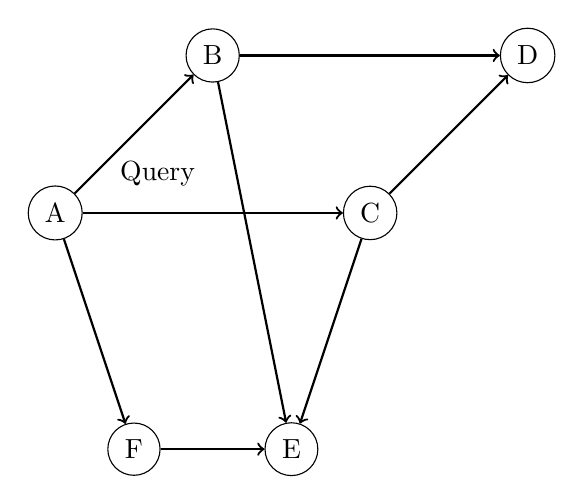
\begin{tikzpicture}
        \node[draw, circle] (A) at (0,0) {A};
        \node[draw, circle] (B) at (2,2) {B};
        \node[draw, circle] (C) at (4,0) {C};
        \node[draw, circle] (D) at (6,2) {D};
        \node[draw, circle] (E) at (3,-3) {E};
        \node[draw, circle] (F) at (1,-3) {F};
      
        \draw[->, thick] (A) -- (B);
        \draw[->, thick] (A) -- (C);
        \draw[->, thick] (B) -- (D);
        \draw[->, thick] (C) -- (D);
        \draw[->, thick] (B) -- (E);
        \draw[->, thick] (C) -- (E);
        \draw[->, thick] (A) -- (F);
        \draw[->, thick] (F) -- (E);
      
        \node at (1.3, 0.5) {Query};
      \end{tikzpicture}
    \caption{Gnutella, an example of unstructured \gls{p2p} network}
    \label{fig:gnutella}
\end{figure}

In this example, peer $A$ sends a query to its neighbors $B$, $C$, and $F$.
Each of these neighbors forwards the query to their own neighbors, resulting in an exponential increase in the number of peers queried.
If peer $E$ has the requested resource, it will respond to the query.
Otherwise, the query continues to propagate through the network until the resource is found or the query's \gls{ttl} expires.

\subsubsection*{Real-World Applications}
One example of an unstructured \gls{p2p} system is the Freenet network.
Freenet is designed to provide anonymous and censorship-resistant data storage and retrieval.
In this system, nodes contribute storage space and bandwidth, and data is distributed across the network without any centralized control.
Nodes communicate with each other to store and retrieve files based on a key-based routing mechanism.
However, there is no predetermined structure or organization of nodes; instead, each node dynamically finds neighbors and routes requests through them.
This unstructured approach enhances the anonymity and resilience of the network, making it difficult for any single entity to control or censor the content (\cite{Clarke2001}).

Another example of an unstructured \gls{p2p} system is the Kazaa network.
Kazaa was a popular file-sharing network where users could share and download various types of files, such as music, videos, and software.
In Kazaa, nodes connect randomly to other nodes without a central directory or predefined organization, forming a loosely structured network.
When a user searches for a file, the search request is propagated through the network to find nodes that have the desired file.
This results in a decentralized and flexible system, but it can lead to high network traffic and inefficiency in locating specific files (\cite{liang2005kazaa}).
Despite these challenges, Kazaa's unstructured nature provided robustness and allowed for a large and dynamic user base.


\subsubsection*{Advantages and Challenges}
Unstructured \gls{p2p} systems offer several advantages.
Their simplicity makes them easy to implement and deploy, and their ad-hoc connectivity allows for high resilience to node failures and network churn.
Since there is no central authority, these networks are highly robust and can continue functioning even when many nodes join or leave the network.
Additionally, the lack of a rigid structure allows for flexible resource sharing and dynamic peer participation.

However, unstructured \gls{p2p} systems face significant challenges, primarily related to the efficiency of resource discovery.
The flooding mechanism used for query propagation can result in high network traffic and slow query resolution times, especially in large networks.
This inefficiency can be mitigated to some extent by techniques such as query caching and intelligent forwarding, but these solutions add complexity to the system.
Moreover, unstructured networks do not guarantee that all resources can be found, as the random topology may lead to disconnected sub-networks where some resources are not reachable from certain peers.

\subsection*{Structured \gls{p2p} Networks}
Structured \gls{p2p} systems represent an advanced and efficient method of managing distributed networks.
Unlike unstructured \gls{p2p} systems, which rely on random connections and flooding-based search techniques, structured \gls{p2p} systems employ a deterministic approach to data placement and retrieval.
This deterministic approach ensures that resources can be found and accessed with predictable efficiency, typically scaling logarithmically with the number of nodes in the network.

The architecture of structured \gls{p2p} systems revolves around the concept of a \gls{dht}.
A \gls{dht} is a decentralized data structure that provides a lookup service similar to a traditional hash table.
Key-value pairs are stored within the \gls{dht}, and any node in the network can retrieve the value associated with a specific key.
The primary operations supported by a \gls{dht} are insertion, lookup, and deletion of key-value pairs.

Hashing is the fundamental operation in a \gls{dht}, responsible for mapping keys to a fixed-size identifier space.
Typically, a cryptographic hash function $H$ is employed to ensure uniform distribution of keys.
Each node in the network is assigned a number (called ``identifier'' or ID) on a ring using a hash function.
Each ID has $m$ bits; there are $2^m$ IDs available and the IDs range from 0 to $(2^m) -1$.

BitTorrent is a widely used \gls{p2p} protocol that leverages structured overlays for efficient content distribution (\cite{BitTorrent2005}).

BitTorrent is an example of unstructured \gls{p2p} system but in an alternative implementation, a node also joins a separate structured \gls{p2p} system like \gls{dht} to facilitate the lookup of peers that hold pieces of the desired content.
When a user wants to download a file, BitTorrent breaks the file into smaller pieces, and peers exchange these pieces with each other.
To efficiently locate which peers have which pieces, BitTorrent uses a \gls{dht}.

Moreover, in BitTorrent, the \gls{dht} is used to store and retrieve metadata about torrents.
The metadata includes information about which peers possess which pieces of the file.
When a peer joins the network, it announces its presence by publishing its information in the \gls{dht} using a key derived from the torrent's identifier.
Other peers looking for that particular torrent can query the \gls{dht} using the same key to find the list of peers holding the pieces of the file.

Fig. \ref{fig:BitTorrent} illustrates how the \gls{dht} in BitTorrent operates during a lookup process:
\begin{figure}[htbp]
    \centering
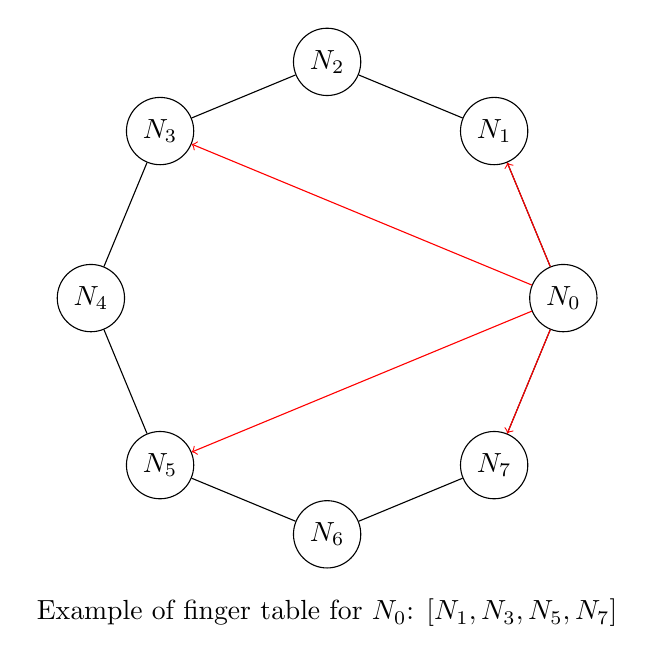
\begin{tikzpicture}
  % Nodes on the ring
  \foreach \i in {0,1,...,7} {
    \node[circle, draw, minimum size=0.8cm] (n\i) at (\i*45:3cm) {$N_\i$};
  }
  % Connections between nodes
  \foreach \i/\j in {0/1, 1/2, 2/3, 3/4, 4/5, 5/6, 6/7, 7/0} {
    \draw[-] (n\i) -- (n\j);
  }
  % Finger table connections for a sample node (N0)
  \draw[->, red] (n0) -- (n1);
  \draw[->, red] (n0) -- (n3);
  \draw[->, red] (n0) -- (n5);
  \draw[->, red] (n0) -- (n7);
  \node at (0,-4) {Example of finger table for $N_0$: [$N_1, N_3, N_5, N_7$]};
\end{tikzpicture}
\caption{BitTorrent, an example of unstructured \gls{p2p} network.}
\label{fig:BitTorrent}
\end{figure}

In this example, node $N_0$ has a finger table containing nodes $N_1, N_3, N_5$ and $N_7$.
When $N_0$ wants to find a key (representing a torrent or a peer holding pieces of a torrent), it consults its finger table to determine the closest preceding node and forwards the query until it reaches the node responsible for the key.
This ensures that the lookup operation is performed efficiently, typically within $\mathcal{O}(\log n)$ hops.
Finger tables have been mentioned in this example, without spontaneously explaining what they are and what they are used for.
A full explanation of them can be found in Section \ref{sec:finger-tables}.

\subsubsection*{Real-World Applications}
Structured \gls{p2p} systems have found application in various domains due to their efficiency and scalability.
Some notable real-world applications include \glspl{cdn}, distributed storage systems, and \gls{dns}.
Systems like BitTorrent utilize structured overlays to efficiently locate and distribute files among peers (\cite{cohen2003incentives}).
The structured approach ensures that pieces of a file can be found and downloaded quickly, even as peers join and leave the network.
Amazon's Dynamo, a highly available key-value store, leverages \glspl{dht} to manage data replication and partitioning (\cite{DeCandia2007}).
Dynamo's architecture ensures that data is evenly distributed across nodes and can be retrieved even in the presence of node failures.
The Coral \gls{cdn} uses a structured \gls{p2p} system to implement a decentralized \gls{dns} service, improving robustness and scalability (\cite{CoralCDN2010}).

\subsubsection*{Advantages and Challenges}
Structured \gls{p2p} systems offer several advantages that make them suitable for large-scale distributed applications.
The deterministic nature of \glspl{dht} ensures that data can be located within a bounded number of hops, typically $\mathcal{O}(\log n)$, where $n$ is the number of nodes in the network.
These systems can scale to accommodate a large number of nodes without significant degradation in performance.
The use of consistent hashing ensures even distribution of data and load across nodes.
Moreover, these systems are designed to handle node churn gracefully.
When nodes join or leave the network, only a small fraction of the keys need to be redistributed, minimizing disruption.

Despite their advantages, structured \gls{p2p} systems face several challenges.
Maintaining the structured overlay network requires nodes to frequently update their routing tables, especially in high-churn environments.
This can introduce overhead and complexity.
Additionally, structured \gls{p2p} systems are vulnerable to various attacks, such as Sybil attacks, where an adversary creates multiple identities to control a significant portion of the network.
Ensuring secure and trustable node identities is crucial.
Although consistent hashing helps distribute data evenly, hotspots can still occur.
Nodes with identifiers close to popular keys may experience higher loads, necessitating additional mechanisms for load balancing.

\section{Unstructured vs Strucuted \gls{p2p} Systems}
The comparison between unstructured and structured \gls{p2p} systems reveals significant differences in various aspects such as scalability, reliability, transparency and load balancing, complexity, security, data consistency, resource discovery, and performance.

Structured \gls{p2p} systems are designed with scalability in mind.
They use deterministic algorithms and \glspl{dht} to manage resources efficiently.
This allows them to grow significantly without a proportional increase in the time required to locate resources, as the lookup time typically scales logarithmically with the number of nodes in the network, denoted as \(\mathcal{O}(\log N)\).
In contrast, unstructured \gls{p2p} systems rely on techniques like flooding or random walks for resource discovery, which can lead to significant scalability issues.
As the network expands, the number of messages required to find resources increases dramatically, causing network congestion and higher latency.

Reliability is another domain where structured \gls{p2p} systems excel.
Their structured nature and the use of \glspl{dht} ensure an even distribution of data across nodes and efficient handling of node joins and departures with minimal data movement.
Additionally, redundancy and data replication in structured systems further enhance reliability.
On the other hand, unstructured \gls{p2p} systems often depend on a small subset of nodes for resource availability.
This reliance can lead to reliability problems, especially if key nodes leave the network, potentially resulting in data loss or inaccessible resources.

In terms of transparency and load balancing, structured \gls{p2p} systems offer inherent advantages.
The \gls{dht} mechanism ensures that data is evenly distributed across all nodes, preventing hotspots and ensuring uniform load distribution.
In contrast, unstructured \gls{p2p} systems lack built-in load balancing mechanisms, leading to potential performance issues.
Popular nodes or resources can become overwhelmed, causing performance degradation unless additional overlays or mechanisms are introduced.

However, structured \gls{p2p} systems come with higher complexity.
Implementing and maintaining these systems require sophisticated algorithms for consistent hashing, overlay maintenance, and efficient routing.
Regular updates to routing tables and handling edge cases add to this complexity.
Unstructured \gls{p2p} systems are simpler to implement as they do not require a predefined structure or complex routing algorithms.
Nodes can join and leave the network with minimal overhead, making these systems easier to manage, although this simplicity comes at the cost of efficiency and performance.

Security is a critical consideration in \gls{p2p} systems.
Structured \gls{p2p} systems can be more secure due to their predictable structure and the use of cryptographic techniques in \glspl{dht}.
Nonetheless, they remain vulnerable to specific attacks such as the Sybil attack, where an adversary inserts multiple nodes to disrupt the network.
Unstructured \gls{p2p} systems, due to their lack of structure, are more susceptible to security threats.
These systems are particularly vulnerable to denial-of-service attacks and the insertion of malicious nodes, which can severely disrupt resource discovery and compromise data integrity.

Data consistency is another area where structured \gls{p2p} systems perform better.
The deterministic data placement ensures that updates are consistently propagated to all replicas, maintaining data integrity.
In unstructured \gls{p2p} systems, maintaining data consistency is more challenging due to the random replication of data across nodes.
Ensuring that all replicas are updated consistently requires additional, often complex, protocols.

Resource discovery in structured \gls{p2p} systems is efficient and predictable.
The use of \glspl{dht} ensures that any resource can be located within a logarithmic number of hops, making these systems suitable for applications requiring quick and reliable resource access.
In unstructured \gls{p2p} systems, resource discovery is less efficient, as nodes typically rely on flooding or random walks, leading to high latency and incomplete searches, particularly in larger networks.

Performance is generally better in structured \gls{p2p} systems due to the efficient resource discovery and data retrieval mechanisms.
The logarithmic scaling of lookup operations ensures that performance remains acceptable even as the network grows.
Unstructured \gls{p2p} systems can suffer from poor performance due to the inefficiency of their resource discovery methods.
Extensive message passing and potential network congestion can slow down resource retrieval times significantly.

In conclusion, structured \gls{p2p} systems offer several advantages over unstructured systems, including better scalability, reliability, load balancing, and performance.
They provide efficient resource discovery and maintain data consistency effectively.
However, these benefits come at the cost of increased complexity and implementation overhead.
Unstructured \gls{p2p} systems, while simpler and easier to deploy, face significant challenges in terms of scalability, reliability, and performance, making them less suitable for large-scale applications.
The choice between structured and unstructured \gls{p2p} systems ultimately depends on the specific requirements of the application, such as the need for efficiency, reliability, and scalability.
\fillingPage{}
\chapter{Chord Architecture}\label{chap:chord}
The Chord protocol is designed to address the challenges of efficient resource discovery and management in \gls{p2p} systems.
It provides a robust and scalable solution for locating nodes and data in a distributed network.
Chord organizes nodes in a circular identifier space using consistent hashing.
Each node and data item is assigned a unique identifier, ensuring uniform distribution across the identifier space.

\section{Node Identifiers and Consistent Hashing}
Chord uses a consistent hash function, such as SHA-1, to generate identifiers for nodes and data items.
These identifiers are arranged in a circular space, often referred to as an identifier ring.
The position of each node and data item on this ring is determined by their hash value (\cite{stoica2001}).

Entities in a Chord \gls{dht} are represented as key-value pairs, where the key denotes the entity's name and the value indicates its address.
A hash function $H$ is used to map both the entity key and the node address to an identifier space.
\begin{itemize}
    \item $H(\text{key})$ is the entity identifier;
	\item $H(\text{address})$ is the node identifier.
\end{itemize}

Chord \gls{dht} operates within an $m$-bit circular identifier space, which means it can accommodate $2^m$ unique identifiers.
An entity with identifier $e$ is stored on the node with identifier $n$ if $n \geq e$.
In that case, this node $n$ is referred to as the \textbf{successor} of $e$.

In Fig. \ref{fig:chord-ring-nodes-entities}, $m$ is set to 3, creating an identifier space with $2^3$ values, ranging from 0 to 7 inclusive.
The nodes are identified by 2, 5, and 7, with the remaining identifiers representing entities.
The list below shows which nodes are responsible for which entities:
\begin{itemize}
    \item Node 2: Entity 0, Entity 1, and Entity 2;
	\item Node 5: Entity 3, Entity 4, and Entity 5;
	\item Node 7: Entity 6 and Entity 7.
\end{itemize}
	
\begin{figure}[htbp]
    \centering
    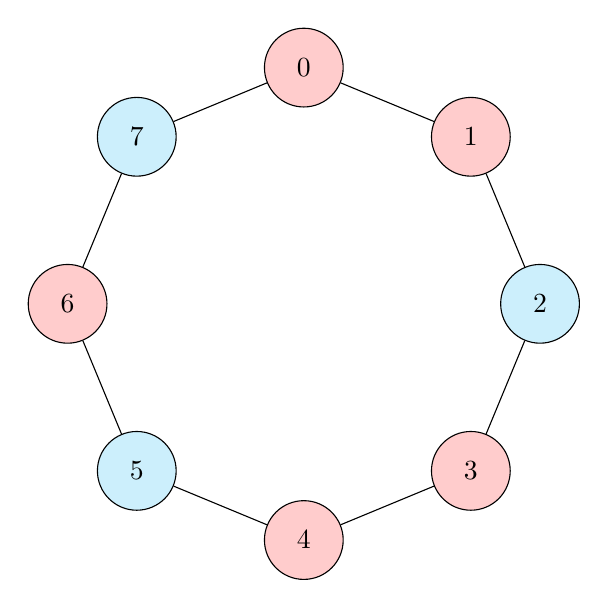
\begin{tikzpicture}

        % Define the number of circles and the radius of the ring
        \def\n{8}
        \def\radius{3}
        
        % Loop to draw the circles in a ring and add labels
        \foreach \i in {0,...,7} {
            \pgfmathsetmacro{\angle}{90 - \i * 360 / \n}
            \ifnum\i=0 \node[circle, draw, fill=red!20, minimum size=1cm] (C\i) at (\angle:\radius) {\i};
            \else\ifnum\i=1 \node[circle, draw, fill=red!20, minimum size=1cm] (C\i) at (\angle:\radius) {\i};
            \else\ifnum\i=3 \node[circle, draw, fill=red!20, minimum size=1cm] (C\i) at (\angle:\radius) {\i};
            \else\ifnum\i=4 \node[circle, draw, fill=red!20, minimum size=1cm] (C\i) at (\angle:\radius) {\i};
            \else\ifnum\i=6 \node[circle, draw, fill=red!20, minimum size=1cm] (C\i) at (\angle:\radius) {\i};
            \else\ifnum\i=2 \node[circle, draw, fill=cyan!20, minimum size=1cm] (C\i) at (\angle:\radius) {\i};
            \else\ifnum\i=5 \node[circle, draw, fill=cyan!20, minimum size=1cm] (C\i) at (\angle:\radius) {\i};
            \else \node[circle, draw, fill=cyan!20, minimum size=1cm] (C\i) at (\angle:\radius) {\i};
            \fi\fi\fi\fi\fi\fi\fi
        }
        
        % Loop to draw round links between each pair of adjacent circles
        \foreach \i in {0,...,7} {
            \pgfmathtruncatemacro{\nexti}{mod(\i+1,8)}
            \draw [rounded corners] (C\i) -- (C\nexti);
        }
        
        \end{tikzpicture}
    \caption{Chord ring with 8 nodes. Blue nodes represent data items, while red nodes represent Chord nodes.}
    \label{fig:chord-ring-nodes-entities}
\end{figure}

\section{Finger Tables}\label{sec:finger-tables}
For peers in a Chord network to locate each other, each peer must be aware of at least one other peer in the network.
Specifically, each peer needs to know the IP address (along with the TCP or UDP port) of their nearest neighbor in terms of identifier in the Chord network.
\begin{figure}[htbp]
    \centering
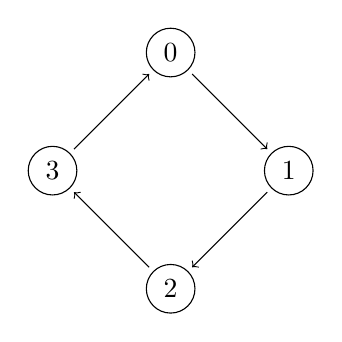
\begin{tikzpicture}
    % Define the positions of the nodes in a ring with shorter arrows
    \node[circle, draw] (0) at (90:1.5) {0};
    \node[circle, draw] (1) at (0:1.5) {1};
    \node[circle, draw] (2) at (270:1.5) {2};
    \node[circle, draw] (3) at (180:1.5) {3};
    
    % Draw the directional arrows between the nodes with shorter distances
    \draw[->, shorten >=2pt, shorten <=2pt] (0) -- (1);
    \draw[->, shorten >=2pt, shorten <=2pt] (1) -- (2);
    \draw[->, shorten >=2pt, shorten <=2pt] (2) -- (3);
    \draw[->, shorten >=2pt, shorten <=2pt] (3) -- (0);
\end{tikzpicture}
\caption{Chord ring with 4 nodes. Each node is aware of its immediate neighbors.}
\label{fig:chord-ring-peer-neighbours}
\end{figure}

This is illustrated in the Fig. \ref{fig:chord-ring-peer-neighbours}, where each node is aware of its immediate neighbors.

By knowing only the nearest neighboring peer in the network, it is still possible to find any peer.
The lookup algorithm works as follows:
\begin{enumerate}
    \item If the nearest neighbor is the peer (ID) we are looking for, the lookup is successful;
	\item Else, ask the nearest neighbor to return either the address of the target peer or the closest peer it knows to the target peer, if it doesn't know the target peer itself;
	\begin{itemize}
        \item If the returned peer (ID) is the peer we are looking for, the lookup is successful.
        \item If the neighboring peer does not know any peer closer to the target peer than itself, it returns no peer info, and the lookup is unsuccessful.
        \item Else, repeat step 2 by sending the request to the peer returned from the previous lookup request.
    \end{itemize}
\end{enumerate}

Using this simple algorithm, the searching peer will eventually query all peers in the network, one at a time, until it finds the target peer or concludes that the closest peer it knows is itself, which will occur after a complete round in the network.

However, only relying on the nearest neighbor results in a lookup time of $\mathcal{O}(N)$, meaning the lookup time increases linearly with the number of peers in the Chord network.
Chord addresses this problem with a more efficient solution.
\\To improve lookup times, the Chord finger table (also called routing table) is structured so that each peer maintains pointers (entries) to more than just their nearest neighbor in the Chord network.
The finger table of a node \(n\) contains up to \(m\) entries, where \(m\) is the number of bits in the identifier.
The $i-$th entry in the finger table of node \(n\) points to the first node that succeeds \(n + 2^{i-1}\) on the identifier circle.
This allows nodes to efficiently route queries by skipping intermediate nodes and reducing the number of hops (\cite{stoica2001}).
In other words, finger tables accelerate the lookup process in a Chord \gls{dht} by containing shortcuts to existing nodes in the ring, thereby reducing the distance traveled during the search for a particular node.
Each node has a finger table with the addresses of $m$ successive nodes, which is used to navigate to other nodes during lookup.
Here are some syntactical details of these finger tables commonly used in Chord \gls{dht} algorithms:
\begin{itemize}
    \item $FT_n$ represents the finger table for node $n$.
    For example, $FT_1$ refers to the finger table of node 1.
	\item $FT_n[i]$ represents the $i$-th successor of node $n$.
    For example, $FT_1[2]$ refers to the second successor node in the finger table of node 1.
\end{itemize}
Table \ref{tab:peer-finger-table} shows $FT_3$, the finger table for a peer with ID 3 in a Chord network with 8-bit IDs.
\begin{table}[htbp]
    \centering
    \begin{tabular}{|c|c|c|}
        \hline
        \textbf{Entry Index} & \textbf{Referenced ID} & \textbf{ID Distance} \\ \hline
        0 & 4 & $1 \ (2^0)$ \\ \hline
        1 & 5 & $2 \ (2^1)$ \\ \hline
        2 & 7 & $4 \ (2^2)$ \\ \hline
        3 & 11 & $8 \ (2^3)$ \\ \hline
        4 & 19 & $16 \ (2^4)$ \\ \hline
        5 & 35 & $32 \ (2^5)$ \\ \hline
        6 & 67 & $64 \ (2^6)$ \\ \hline
        7 & 131 & $128 \ (2^7)$ \\ \hline
    \end{tabular}
    \caption{A peer finger table for peer with ID 3 (8 bit ID size).}
    \label{tab:peer-finger-table}
\end{table}

The first 4 references of the peer with ID 3 are illustrated in Fig. \ref{fig:chord-ring-16-peers-4-references-peer-3}.
It provides a sense of how the exponentially increasing distances of references appear in a virtual Chord ring:

\begin{figure}[htbp]
    \centering
    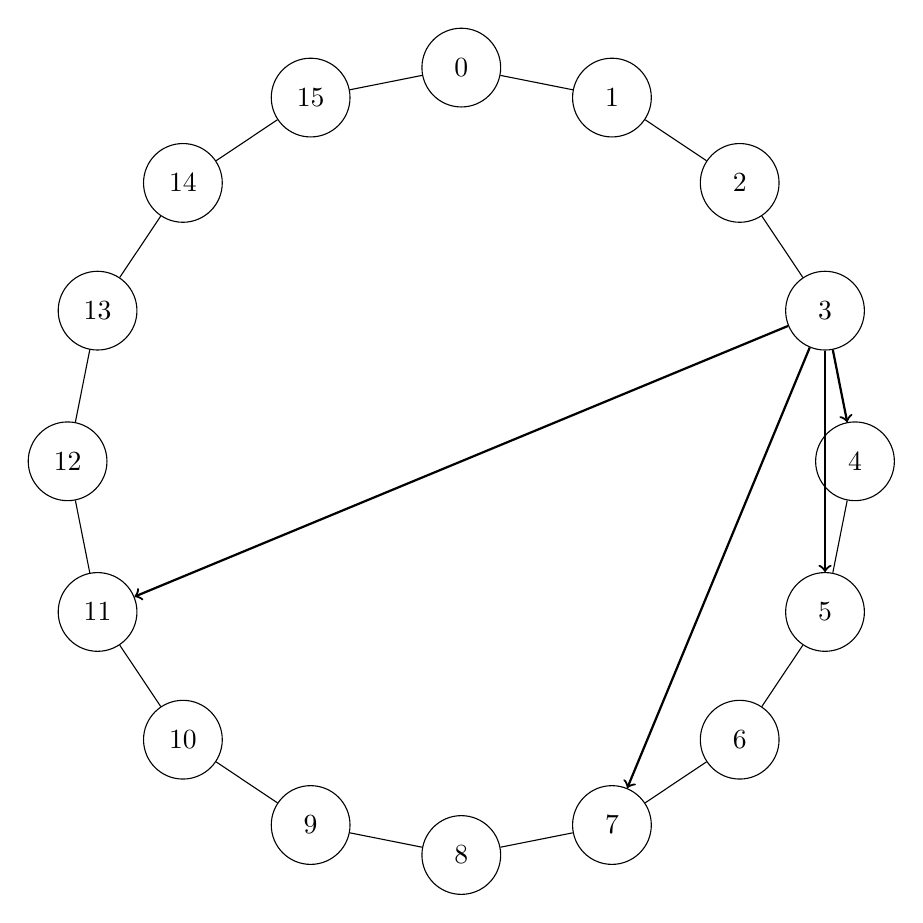
\begin{tikzpicture}

        % Define the number of circles and the radius of the ring
        \def\n{16}
        \def\radius{5}
        
        % Loop to draw the circles in a ring and add labels
        \foreach \i in {0,...,15} {
            \pgfmathsetmacro{\angle}{90 - \i * 360 / \n}
            \node[circle, draw, fill=white, minimum size=1cm] (C\i) at (\angle:\radius) {\i};
        }
        
        % Loop to draw round links between each pair of adjacent circles
        \foreach \i in {0,...,15} {
            \pgfmathtruncatemacro{\nexti}{mod(\i+1,16)}
            \draw [rounded corners] (C\i) -- (C\nexti);
        }

        % Draw additional directional arrows from node 3 to nodes 4, 5, 7, and 11
        \draw[->, thick] (C3) -- (C4);
        \draw[->, thick] (C3) -- (C5);
        \draw[->, thick] (C3) -- (C7);
        \draw[->, thick] (C3) -- (C11);
        
    \end{tikzpicture}
    \caption{Chord ring with 16 peers. The first 4 references of the peer with ID 3 are represented by the arrows.}
    \label{fig:chord-ring-16-peers-4-references-peer-3}
\end{figure}

\section{Lookups and Routing}
As explained in the previous section, when a node needs to locate a data item, it generates the identifier for the item using the hash function $H$.
The node then uses its finger table to forward the query to the appropriate node responsible for the identifier.
This process continues iteratively, with each node forwarding the query closer to the target node, until the node responsible for the data item is found.
The expected number of hops for a lookup is \(O(\log N)\) (\cite{stoica2001}).

\section{Chord Lookup Example}
To better understand how the Chord lookup algorithm works, let's examine a lookup example.
In this scenario, the peer with ID 3 needs to locate the peer with ID 2.

Firstly, here are the finger tables for the peers involved in this specific lookup (peers 3, 11, 15, and 1):
\begin{figure}[htbp]
    \centering
    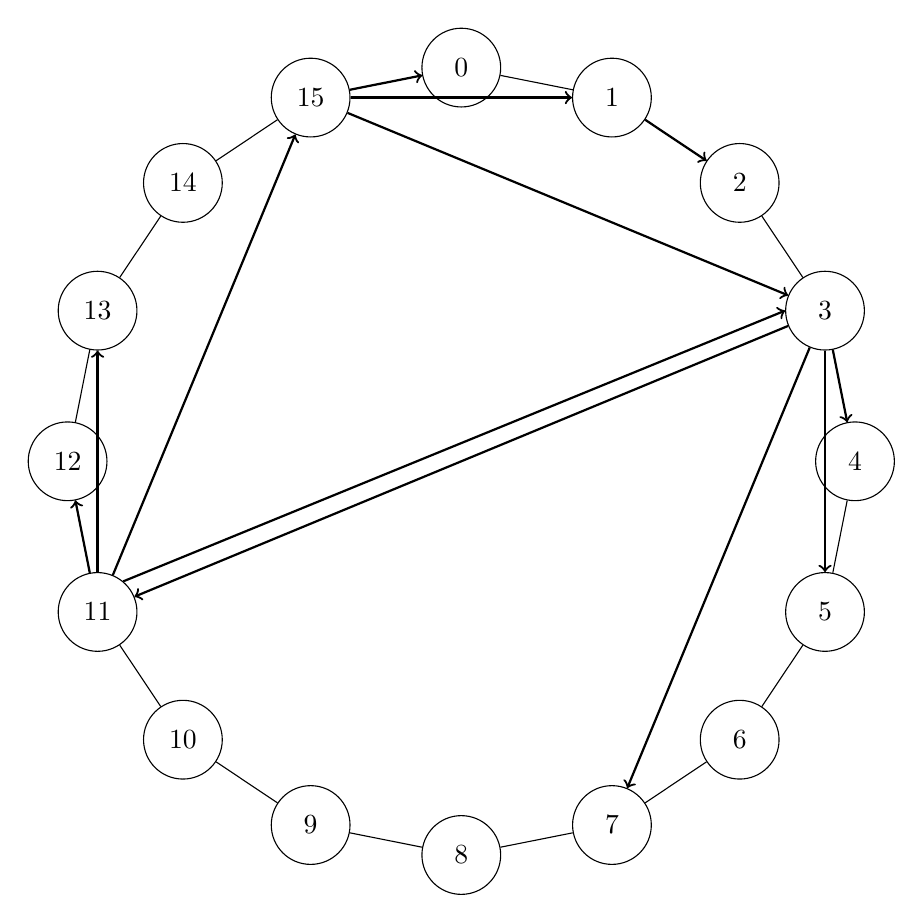
\begin{tikzpicture}

        % Define the number of circles and the radius of the ring
        \def\n{16}
        \def\radius{5}
        
        % Loop to draw the circles in a ring and add labels
        \foreach \i in {0,...,15} {
            \pgfmathsetmacro{\angle}{90 - \i * 360 / \n}
            \node[circle, draw, fill=white, minimum size=1cm] (C\i) at (\angle:\radius) {\i};
        }
        
        % Loop to draw round links between each pair of adjacent circles
        \foreach \i in {0,...,15} {
            \pgfmathtruncatemacro{\nexti}{mod(\i+1,16)}
            \draw [rounded corners] (C\i) -- (C\nexti);
        }

        % Draw additional directional arrows from node 3 to nodes 4, 5, 7, and 11
        \draw[->, thick] (C3) -- (C4);
        \draw[->, thick] (C3) -- (C5);
        \draw[->, thick] (C3) -- (C7);
        \draw[->, thick] (C3) -- (C11);
        \draw[->, thick] (C11) -- (C12);
        \draw[->, thick] (C11) -- (C13);
        \draw[->, thick] (C11.50) -- (C3.180);
        \draw[->, thick] (C11) -- (C15);
        \draw[->, thick] (C15) -- (C0);
        \draw[->, thick] (C15) -- (C1);
        \draw[->, thick] (C15) -- (C3);
        \draw[->, thick] (C1) -- (C2);
        
    \end{tikzpicture}
    \caption{Chord lookup example.}
    \label{fig:chord-ring-16-peers-lookup-example}
\end{figure}

The lookup process proceeds as follows:
\begin{enumerate}
    \item The peer with ID 3 first examines its own finger table and identifies the peer with the closest ID to 2, which is the peer with ID 11;
	\item The searching peer then contacts the peer with ID 11 and inquires about the closest peer it knows to the peer with ID 2. The peer with ID 11 points to the peer with ID 15;
	\item Next, the searching peer contacts the peer with ID 15 and asks for the closest peer it knows to the peer with ID 2. The peer with ID 15 points to the peer with ID 1;
	\item The searching peer then contacts the peer with ID 1 and asks for the closest peer it knows to the peer with ID 2. The peer with ID 1 points to the peer with ID 2.
\end{enumerate}

The lookup is now complete.

These steps are illustrated in Fig. \ref{fig:chord-example-lookup-steps}. The red arrows indicate the lookup progression.

\begin{figure}[htbp]
    \centering
    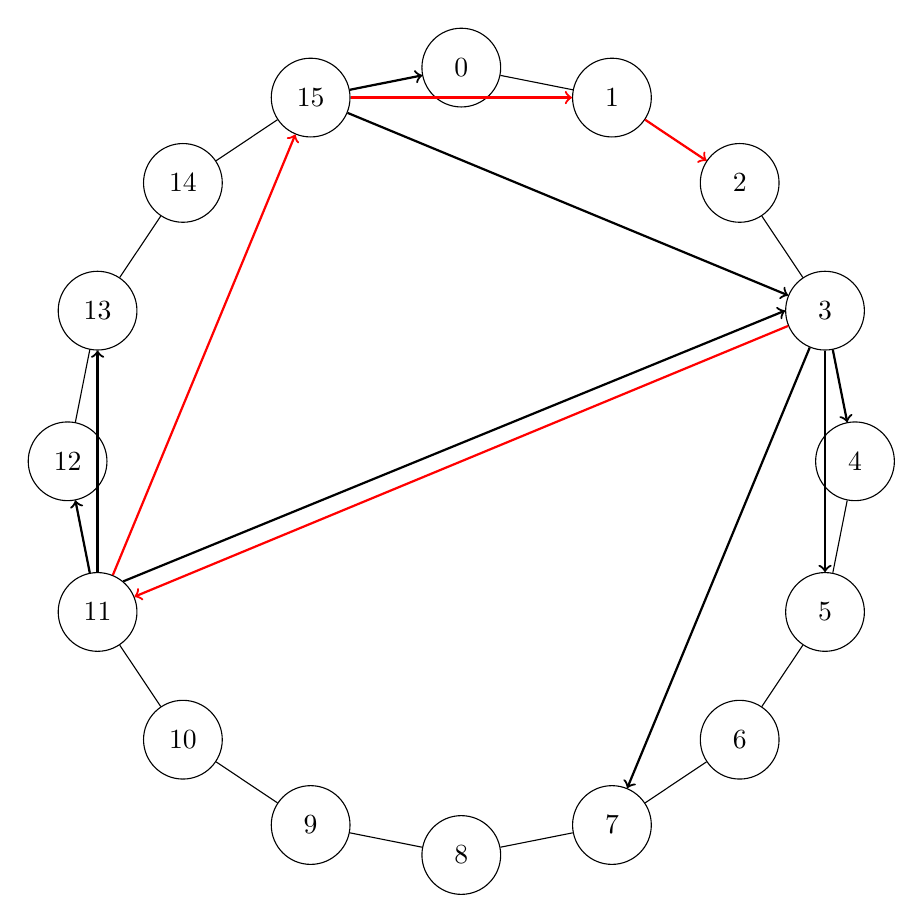
\begin{tikzpicture}

        % Define the number of circles and the radius of the ring
        \def\n{16}
        \def\radius{5}
        
        % Loop to draw the circles in a ring and add labels
        \foreach \i in {0,...,15} {
            \pgfmathsetmacro{\angle}{90 - \i * 360 / \n}
            \node[circle, draw, fill=white, minimum size=1cm] (C\i) at (\angle:\radius) {\i};
        }
        
        % Loop to draw round links between each pair of adjacent circles
        \foreach \i in {0,...,15} {
            \pgfmathtruncatemacro{\nexti}{mod(\i+1,16)}
            \draw [rounded corners] (C\i) -- (C\nexti);
        }

        % Draw additional directional arrows from node 3 to nodes 4, 5, 7, and 11
        \draw[->, thick] (C3) -- (C4);
        \draw[->, thick] (C3) -- (C5);
        \draw[->, thick] (C3) -- (C7);
        \draw[->, thick, red] (C3) -- (C11);
        \draw[->, thick] (C11) -- (C12);
        \draw[->, thick] (C11) -- (C13);
        \draw[->, thick] (C11.50) -- (C3.180);
        \draw[->, thick, red] (C11) -- (C15);
        \draw[->, thick] (C15) -- (C0);
        \draw[->, thick, red] (C15) -- (C1);
        \draw[->, thick] (C15) -- (C3);
        \draw[->, thick, red] (C1) -- (C2);
        
    \end{tikzpicture}
    \caption{Example of Chord lookup steps.}
    \label{fig:chord-example-lookup-steps}
\end{figure}

\section{Joining and Leaving the Network}
When a new node joins the Chord network, it must integrate into the existing structure.
The joining node needs to initialize its finger table and notify other nodes of its presence.
This involves updating the finger tables of existing nodes to reflect the new node's position.
The new node first contacts an existing node in the network to find its appropriate position in the identifier circle.
Once its position is determined, the new node initializes its finger table by querying other nodes for the necessary information.

The joining process also requires the new node to transfer relevant data from its predecessor, ensuring that data responsibility is correctly assigned.
Additionally, the new node must notify its predecessor and successor about its presence, prompting them to update their respective finger tables.
This notification process may propagate further updates across the network to maintain the integrity and efficiency of the lookup process.

When a node leaves the network, it must transfer its data to its successor node and notify other nodes to update their finger tables accordingly.
The departing node first ensures that all its data is transferred to its immediate successor, guaranteeing no data loss occurs.
Following the data transfer, the leaving node informs its predecessor and successor, as well as potentially other nodes, to adjust their finger tables to exclude the departing node.

Chord's protocol is designed to handle frequent join and leave operations seamlessly, ensuring the network remains robust and efficient.
This self-healing capability of the Chord network allows it to maintain consistent data availability and efficient routing performance.
The protocol dynamically adjusts the finger tables and data responsibilities, minimizing the impact of node churn on the overall system.

Furthermore, Chord uses stabilization protocols that periodically run to correct any inconsistencies in the finger tables and ensure all nodes have accurate and up-to-date routing information.
These stabilization routines help in maintaining the correctness and performance of the network despite the continuous changes in its composition.

By effectively managing the joining and leaving of nodes, Chord ensures that the \gls{dht} structure remains functional, providing a scalable and resilient platform for distributed applications.

Chord's ability to adapt to the dynamic nature of \gls{p2p} networks, where nodes frequently join and leave, highlights its efficiency and reliability.
The protocol's mechanisms for updating finger tables and redistributing data ensure that the network can sustain a high degree of availability and performance, which are crucial for the practical deployment of distributed systems (\cite{stoica2001}).

\section{Advantages and Limitations}
One of the primary advantages of Chord is its scalability.
The protocol can efficiently manage a large number of nodes, ensuring that as the number of nodes grows, the number of steps required to find a particular data item increases logarithmically.
This property makes Chord highly suitable for applications requiring dynamic and scalable networks, such as \gls{p2p} systems (\cite{stoica2001}).
Additionally, Chord provides a decentralized approach, eliminating the need for a central coordinator, which enhances fault tolerance and reduces single points of failure.
Each node in the network maintains only a small amount of routing information about other nodes, enabling the network to handle frequent node arrivals and departures without significant disruptions.

Another advantage of Chord is its simplicity and ease of implementation.
The protocol relies on consistent hashing to distribute data across nodes uniformly, which simplifies the process of locating and retrieving data.
This uniform distribution helps in balancing the load among nodes, preventing any single node from becoming a bottleneck (\cite{stoica2001}).
Moreover, Chord's ring structure allows for efficient data retrieval, as each node only needs to know about its successor and a few other nodes in the ring to route queries effectively.

However, Chord also has several disadvantages.
One significant limitation is its reliance on consistent hashing, which, while effective in balancing load, can lead to suboptimal data placement and increased latency in certain scenarios.
For example, if the hash function does not evenly distribute data, some nodes may end up handling more requests than others, leading to uneven load distribution and potential performance bottlenecks (\cite{stoica2001}).
Additionally, Chord's performance can be impacted by network latency and the physical distribution of nodes, as the protocol does not consider the proximity of nodes when routing queries, potentially resulting in longer query times (\cite{balatsouras2022wichord}).

Another disadvantage of Chord is its maintenance overhead.
As nodes frequently join and leave the network, the protocol must constantly update its routing information to maintain consistency and ensure efficient data retrieval.
This maintenance can introduce additional communication overhead and complexity, particularly in highly dynamic environments (\cite{stoica2001}).
Furthermore, while Chord is designed to be fault-tolerant, it still requires mechanisms to handle node failures and recover lost data, which can add to the system's overall complexity and resource requirements.

In conclusion, while the Chord protocol offers significant advantages in terms of scalability, decentralization, and simplicity, it also faces challenges related to data placement, network latency, and maintenance overhead.
These factors must be carefully considered when implementing Chord in distributed systems to ensure optimal performance and reliability.
\fillingPage{}
\chapter{Systems Based on Chord}
Chord's efficient and scalable architecture has inspired the development of various systems and applications in the field of distributed computing and \gls{p2p} networks.
These systems leverage the unique properties of Chord's \gls{dht} to achieve robustness, fault tolerance, and efficient resource discovery.
This chapter explores several notable applications of Chord in different domains, highlighting real-world examples, advantages, disadvantages, and additional details.

\section{File Sharing Systems}
One of the most common applications of Chord is in file-sharing systems.
These systems use Chord's \gls{dht} to store and retrieve files efficiently, ensuring high availability and fault tolerance.
The \gls{cfs} employs Chord to provide a robust and efficient file storage and retrieval service.
It distributes file blocks across multiple nodes, ensuring redundancy and fault tolerance, making it suitable for large-scale file distribution.
\gls{cfs} breaks files into smaller chunks and distributes them across the network to balance the load and enhance data availability.
This approach not only improves access times but also ensures that the system can recover quickly from node failures, maintaining the integrity and availability of stored files (\cite{Dabek2001}).
Large-scale academic repositories and research data sets often use systems similar to \gls{cfs} to ensure data availability and fault tolerance.
The primary advantages of \gls{cfs} include high redundancy, fault tolerance, decentralized control, and scalability.
However, it can suffer from potentially high latency for file retrieval if the network is large or nodes are widely dispersed.

Ivy, a multi-user read/write \gls{p2p} file system, uses Chord for efficient data location, allowing users to collaboratively manage and share files in a decentralized manner (\cite{Ivy2003}).
Ivy supports concurrent file updates and conflict resolution, making it suitable for collaborative environments.
By leveraging Chord's \gls{dht}, Ivy can efficiently locate and manage file metadata, ensuring that users can quickly access the files they need.
This system exemplifies how Chord can be used to build robust, scalable file-sharing solutions that operate without central control.
Ivy-like systems are useful for collaborative projects in distributed teams, such as software development or content creation.
Ivy's main advantages are its support for collaborative file management, efficient metadata handling, and decentralized architecture.
However, conflict resolution can be complex, and there can be potential data inconsistency issues.

\section{Distributed Databases}
Chord's principles have been applied to the design of distributed databases, providing scalable and fault-tolerant data storage solutions.
Dynamo, developed by Amazon, is a distributed key-value store that uses concepts similar to Chord for partitioning and replicating data across multiple nodes.
Dynamo ensures high availability and durability, even in the presence of node failures.
It employs a consistent hashing mechanism to distribute data evenly across nodes, reducing hotspots and ensuring efficient load balancing.
Dynamo's replication and quorum-based techniques allow it to achieve high fault tolerance, making it a cornerstone of Amazon's highly available services (\cite{DeCandia2007}).
Amazon's Dynamo is the core of many of its services, ensuring consistent performance during events like Black Friday sales.
The primary advantages of Dynamo include high availability, fault tolerance, efficient load balancing, and scalability.
However, managing consistency and conflict resolution can be complex, and there is a high overhead for replication and quorum maintenance.

Cassandra is another highly scalable distributed database that employs a Chord-like \gls{dht} for data distribution.
It provides a decentralized and fault-tolerant architecture, making it suitable for large-scale applications.
Cassandra's architecture allows it to handle large amounts of data across many commodity servers, providing high throughput and low latency.
The use of Chord-like principles ensures that data is evenly distributed, enabling efficient query processing and robust data replication (\cite{Lakshman2010}).
Cassandra is used by companies like Facebook, Instagram, and Netflix to manage large-scale data requirements with high availability and low latency.
Its advantages include high scalability, low latency, fault tolerance, and a decentralized architecture.
However, Cassandra's complexity in data modeling and its eventual consistency model can lead to temporary data inconsistency.

\section{\acrlong{cdn}}
Chord's efficient resource discovery and routing capabilities make it a suitable choice for content distribution networks.
Coral is a content distribution network that uses Chord to locate and distribute web content efficiently.
It reduces the load on origin servers and enhances the scalability of content delivery.
By caching web content at various nodes across the network, Coral can quickly serve content to users from the nearest available node, reducing latency and improving user experience.
The Chord \gls{dht} enables efficient location of cached content, ensuring that requests are routed to the most appropriate node (\cite{CoralCDN2010}).
CoralCDN is a real-world example, designed to alleviate the load on websites during traffic spikes.
Coral's advantages include reducing load on origin servers, enhancing scalability, and improving user experience by reducing latency.
However, maintaining cache consistency can be challenging, and there is potential for uneven distribution of content load.

Vuze, a popular BitTorrent client, utilizes Chord to manage its \gls{dht} for peer discovery and content distribution.
It enables efficient sharing and downloading of large files in a decentralized manner.
Vuze leverages Chord to maintain an up-to-date list of peers, facilitating quick and efficient connections between users.
This approach helps distribute the load of file sharing, ensuring that large files can be downloaded quickly and reliably without relying on central servers.
Vuze is widely used for downloading large multimedia files and software distributions.
The main advantages of Vuze include its decentralized nature, efficient peer discovery, scalability, and robustness against failures.
However, there can be potential legal issues with content distribution, and download speeds can vary depending on peer availability.

\section{Distributed Computing}
Chord has also been used in distributed computing platforms to manage and allocate computational resources.
The \gls{boinc} uses Chord-like \glspl{dht} to manage and distribute computational tasks across volunteer nodes.
\gls{boinc} supports large-scale scientific computing projects by leveraging the idle processing power of participant computers.
\gls{boinc}'s use of Chord-like structures ensures efficient task allocation and result collection, enabling it to handle a wide range of scientific computations, from searching for extraterrestrial intelligence to climate modeling (\cite{BOINC2004}).
\gls{boinc} supports various projects like SETI@home, ClimatePrediction.net, and more.
The primary advantages of \gls{boinc} include leveraging idle computing power, supporting a wide range of scientific projects, and its decentralized nature.
However, it depends heavily on volunteer participation, and the availability of computing power can be variable.

SETI@home, a distributed computing project aimed at analyzing radio signals for signs of extraterrestrial intelligence, employs Chord to efficiently distribute and manage data analysis tasks across a global network of volunteer computers (\cite{anderson2002seti}).
By using Chord for task distribution, SETI@home can efficiently allocate computational work to thousands of participants, ensuring that the analysis progresses smoothly and efficiently even as volunteers join and leave the project.
SETI@home is a pioneering example of distributed computing used for scientific research.
Its main advantages include efficient use of distributed resources, engaging the public in scientific research, and scalability.
However, it relies on volunteer computing resources, and there can be data privacy concerns.

\section{Sensor Networks}
WiChord is an adaptation of the Chord protocol designed for \glspl{wsn}, which consist of numerous sensor nodes monitoring environmental conditions.
WiChord addresses the unique challenges of \glspl{wsn}, such as limited energy resources and dynamic network topology, by integrating Chord's \gls{dht}-based architecture with enhancements for energy efficiency and scalability (\cite{balatsouras2022wichord}).

\begin{figure}[htbp]
    \centering
 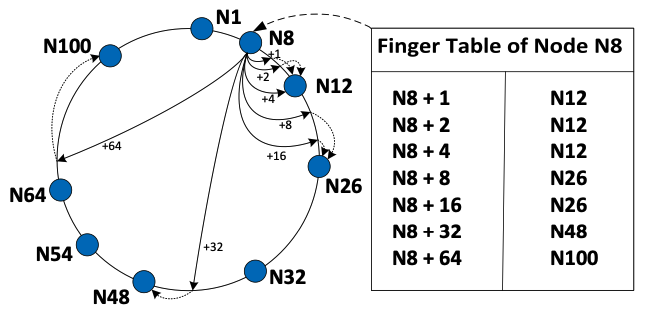
\includegraphics[width=.6\textwidth]{figures/chord-ring-network-sensor-nodes-finger-table.png}
     \rule{35em}{0.5pt}
    \caption{Chord ring network with sensor nodes and finger table in WiChord (\cite{balatsouras2022wichord})} 
\end{figure}


WiChord employs a \gls{dht}-based architecture similar to Chord but optimized for \glspl{wsn}.
It enables efficient data aggregation and query processing by minimizing communication overhead and conserving energy.
Nodes in WiChord aggregate data at intermediate points before forwarding it to the base station, reducing transmissions and extending network lifetime.
Additionally, WiChord optimizes routing paths and minimizes hops needed for data transmission, with nodes capable of entering low-power sleep modes to conserve energy further.
It maintains scalability and fault tolerance, handling the addition and failure of nodes without significant disruption.

\begin{figure}[htbp]
    \centering
 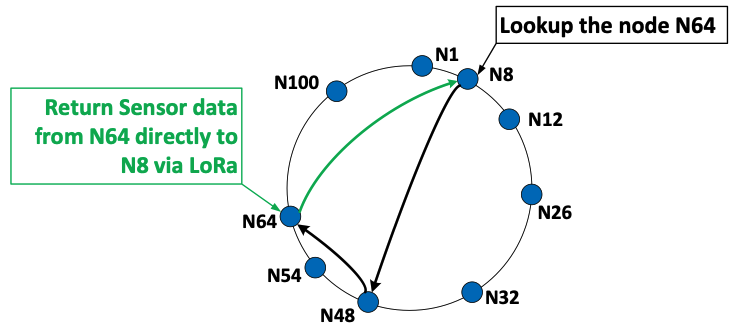
\includegraphics[width=.6\textwidth]{figures/chord-lookup-message-from-one-node-to-another.png}
     \rule{35em}{0.5pt}
    \caption{A lookup message from 2 nodes on a Chord sensor network nodes in WiChord (\cite{balatsouras2022wichord})} 
\end{figure}

WiChord can be applied in various real-world scenarios, including environmental monitoring, smart agriculture, and urban infrastructure monitoring.
For example, in environmental monitoring, WiChord efficiently collects and transmits data from dispersed sensor nodes to detect early signs of forest fires.
In smart agriculture, it supports precision farming by collecting and transmitting data on soil moisture and crop health, aiding farmers in making informed decisions.
In urban infrastructure monitoring, WiChord helps ensure timely maintenance of structures like bridges and buildings by collecting data on structural health indicators.

The primary advantages of WiChord are its energy efficiency, scalability, and robust data aggregation capabilities, making it suitable for long-term deployments in large-scale \glspl{wsn}.
However, the protocol's complexity can make implementation and maintenance challenging, and its performance may be affected by highly dynamic environments.

WiChord exemplifies how the principles of Chord can be adapted to address the specific needs of \glspl{wsn}, providing an efficient and scalable solution for various data aggregation and query processing applications.
\fillingPage{}
\chapter{Conclusion}\label{chap:conclusion}
The Chord framework represents a significant advancement in the design and implementation of \gls{p2p} systems.
Its robust and scalable architecture addresses key challenges in distributed systems, such as efficient resource discovery, fault tolerance, and dynamic node management.
By organizing nodes in a circular identifier space and utilizing finger tables for efficient routing, Chord ensures optimal performance even in large-scale networks.
Chord's influence extends beyond its original design, inspiring the development of various systems and applications in file sharing, distributed databases, content distribution networks, and distributed computing.
Its principles continue to shape the future of decentralized architectures, driving innovation and enhancing the capabilities of distributed systems.

As the field of distributed systems evolves, the Chord framework remains a foundational model for designing scalable, efficient, and resilient \gls{p2p} networks.
Its contributions to the field underscore the importance of decentralized approaches in achieving robust and high-performance distributed systems.
The continuous development and application of Chord in various domains highlight its enduring relevance and potential for future advancements in distributed computing.

%----------------------------------------------------------------------------------------
%	BIBLIOGRAPHY
%----------------------------------------------------------------------------------------

\fillingPage{}
\nocite{*}
\listOfBibliography

%----------------------------------------------------------------------------------------
%	GLOSSARY (if appropriate)
%----------------------------------------------------------------------------------------

% \fillingPage{}
% \listOfGlossary

%----------------------------------------------------------------------------------------
%	ABBREVIATIONS (if appropriate)
%----------------------------------------------------------------------------------------
\fillingPage{}
\listOfAbbreviation

%%----------------------------------------------------------------------------------------
%%	LIST OF FIGURES (optional)
%%----------------------------------------------------------------------------------------

\fillingPage{} 
\listOfFigures

%%----------------------------------------------------------------------------------------
%%	LIST OF TABLES (optional)
%%----------------------------------------------------------------------------------------

\fillingPage{} 
\listOfTables

%----------------------------------------------------------------------------------------
%	THESIS CONTENT - APPENDICES (if appropriate)
%----------------------------------------------------------------------------------------

\appendix % Cue to tell LaTeX that the following 'chapters' are Appendices

% Include the appendices of the thesis as separate files from the Appendices folder
% Uncomment the lines as you write the Appendices

% \fillingPage{} 
% \input{02_Appendices/AppendixA}

% \fillingPage{} 
% \input{02_Appendices/AppendixB}

%\fillingPage{} 
%\input{02_Appendices/AppendixC}

\clearpage % Start a new page

\backmatter

\end{document}  